\documentclass[11pt,a4paper]{article}

\usepackage[utf8]{inputenc}
\usepackage[T1]{fontenc}
\usepackage{lmodern}
\usepackage{microtype}
\usepackage{geometry}
\usepackage{setspace}
\usepackage{parskip}

\geometry{
    left=2.5cm,
    right=2.5cm,
    top=2.5cm,
    bottom=2.5cm
}
\onehalfspacing
\raggedbottom

\usepackage{graphicx}
\usepackage{float}
\usepackage{subcaption}
\graphicspath{{./}{./assets/}{./images/}}

\newcommand{\testimg}[1]{%
    \IfFileExists{assets/#1}{%
        \includegraphics[width=\textwidth]{assets/#1}%
    }{%
        \fbox{\parbox[c][4cm][c]{0.95\textwidth}{\centering\itshape\small (placeholder: assets/#1)}}%
    }%
}

\usepackage{tikz}
\usetikzlibrary{shapes.geometric, shapes.misc, arrows.meta, positioning, calc, automata, quotes, trees, fit, backgrounds, matrix, chains, decorations.pathreplacing}

\usepackage{listings}
\usepackage{xcolor}

\definecolor{codebg}{HTML}{F7F7F7}
\definecolor{codeframe}{HTML}{DDDDDD}
\definecolor{keyword}{HTML}{005FAF}
\definecolor{comment}{HTML}{6A737D}
\definecolor{string}{HTML}{D73A49}
\definecolor{accent}{HTML}{2E7D32}
\definecolor{warn}{HTML}{C62828}

\lstset{
    basicstyle=\ttfamily\footnotesize,
    keywordstyle=\color{keyword}\bfseries,
    commentstyle=\color{comment}\itshape,
    stringstyle=\color{string},
    numbers=left,
    numberstyle=\tiny\color{gray},
    backgroundcolor=\color{codebg},
    frame=single,
    rulecolor=\color{codeframe},
    breaklines=true,
    tabsize=4,
    showstringspaces=false,
    language=C++,
    aboveskip=1em,
    belowskip=1em,
    extendedchars=true,
    inputencoding=utf8,
    literate=%
        {→}{{$\rightarrow$}}1
        {á}{{\'a}}1 {é}{{\'e}}1 {í}{{\'i}}1 {ó}{{\'o}}1 {ú}{{\'u}}1
}

\usepackage{amsmath}
\usepackage{amssymb}

\usepackage{booktabs}
\usepackage{tabularx}
\usepackage{longtable}
\usepackage{etoolbox}
\usepackage{fancyvrb}

\usepackage{hyperref}
\hypersetup{
    colorlinks=true,
    linkcolor=black,
    urlcolor=keyword,
    citecolor=black,
    pdfauthor={Made Branenda Jordhy, Stefani Angeline Oroh, Michael James Liman},
    pdftitle={IF2211 Algorithm Strategy – Laporan Tugas Besar 3}
}

% HEADER/FOOTER
\usepackage{fancyhdr}
\pagestyle{fancy}
\fancyhf{}
\setlength{\headheight}{36pt}
\fancyhead[L]{%
    \small\textnormal{School of Electrical Engineering and Informatics}\\[-1pt]
    \small\textnormal{Institut Teknologi Bandung}%
}
\fancyhead[R]{\IfFileExists{assets/LOGO.png}{
\includegraphics[height=1cm]{assets/LOGO.png}}{}}
\fancyfoot[L]{\small\textnormal{IF2211 Algorithm Strategy}}
\fancyfoot[R]{\small\thepage}
\renewcommand{\headrulewidth}{0.4pt}
\renewcommand{\footrulewidth}{0.2pt}

% TITLE
\title{
    \vspace{-1.5cm}
    {\Large\textsc{IF2211 Algorithm Strategy}}\\[0.35cm]
    {\LARGE\textbf{Pattern Matching in Chromium Browser Extension for Online Gambling Detection}}\\[0.3cm]
    \vspace{-0.3cm}
}
\author{}
\date{\today}

\begin{document}

\maketitle
\thispagestyle{empty}

\begin{figure}[H]
    \centering
    \IfFileExists{assets/Team_cropped.png}{% 
        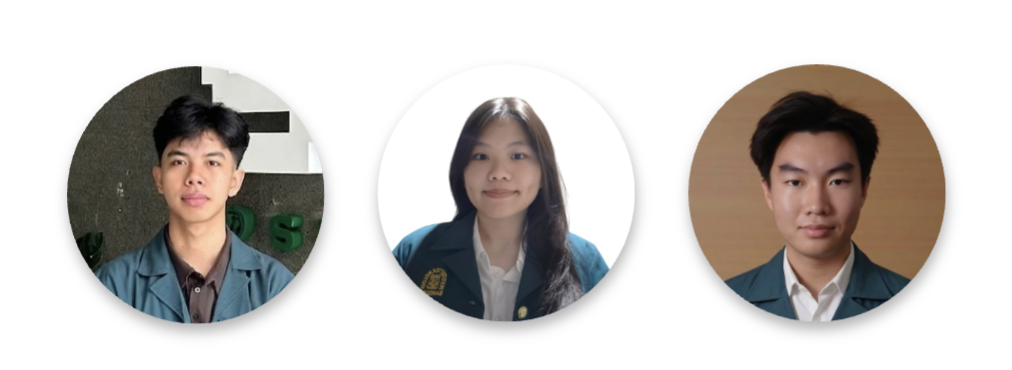
\includegraphics[width=\textwidth,height=0.2\textheight,keepaspectratio]{assets/Team_cropped.png}%
    }{%
        \vspace{4cm}
    }
\end{figure}

\vspace{1cm}
\begin{center}
    \textbf{Made Branenda Jordhy} - 13524026 \\[0.15cm]
    \textbf{Stefani Angeline Oroh} - 13524064 \\[0.15cm]
    \textbf{Michael James Liman} - 13524106 \\[0.15cm]
\end{center}

\vspace{3cm}
\begin{center}
    {\large\textbf{School of Electrical Engineering and Informatics}}\\[0.1cm]
    {\large\textbf{Institut Teknologi Bandung}}\\[0.1cm]
    {\large\textbf{Semester II 2025/2026}}\\[0.1cm]
\end{center}

\newpage
\tableofcontents
\newpage

% =======================================================================
\newpage
\section{Overview}

Proyek ini kami kerjakan untuk memenuhi Tugas Besar 3 mata kuliah IF2211 Strategi Algoritma. Topiknya sudah ditentukan,
yaitu membuat sebuah \textit{Chromium browser extension} yang bisa mendeteksi konten judi online di halaman web, sekaligus
jadi tempat menerapkan algoritma pencocokan string yang dipelajari di kelas.

Topik judol sendiri sebetulnya relevan jika dilihat dari kondisi sekarang. Iklannya ada di mana-mana, mulai dari hasil pencarian
Google, kolom komentar YouTube, sampai sisipan iklan di situs yang sebenarnya tidak ada hubungannya sama sekali dengan perjudian.
Nama-nama yang dipakai pun mirip semua, biasanya berpola \texttt{<kata><angka>} seperti GACOR99, MAXWIN88, atau MADU308, supaya 
gampang diingat dan susah disaring otomatis. Tidak jarang pelakunya juga menyamarkan tulisan dengan karakter yang bentuknya mirip,
misalnya huruf O jadi angka 0, A jadi 4, atau I jadi 1, sehingga filter yang cuma membandingkan string mentah sering kebobolan.

Ekstensi yang kami bangun untuk tugas ini kami beri nama \textbf{Judol Detector}. Begitu halaman selesai dimuat, ekstensi akan
menelusuri DOM, mencocokkan teks dengan daftar kata kunci, lalu menandai elemen yang mengandung kemunculan kata kunci tersebut.
Pengguna bisa mengarahkan kursor ke teks yang ditandai untuk melihat detailnya, atau membuka panel popup ekstensi untuk melihat
ringkasan statistik secara keseluruhan. Pencocokan kata kunci dijalankan dengan beberapa algoritma sekaligus, yaitu Knuth-Morris-Pratt
dan Boyer-Moore untuk tahap pencocokan eksak, RegEx untuk menangkap pola \texttt{<kata><angka>} yang belum tentu ada di daftar kata kunci,
lalu Weighted Levenshtein Distance untuk tahap fuzzy yang menangani kasus penyamaran karakter. Seluruh algoritma string matching
dibuat \textit{from scratch}, tanpa bantuan \texttt{String.includes()}, \texttt{String.indexOf()}, atau pustaka pencocokan string apapun.
Tiap algoritma juga menghitung jumlah perbandingan karakter (\textit{comparison counting}) supaya performanya bisa dibandingkan secara
objektif.

% =======================================================================
\newpage
\section{Theoretical Background}

% =======================================================================
\newpage
\section{Problem Analysis \& Solution Design}

% =======================================================================
\newpage
\section{Implementation \& Testing}

% =======================================================================
\newpage
\section{Conclusion \& Suggestion}

% =======================================================================
\newpage
\begin{thebibliography}{9}

\bibitem{aho2006}
A.~V.~Aho, M.~S.~Lam, R.~Sethi, and J.~D.~Ullman,
\textit{Compilers: Principles, Techniques, and Tools}, 2nd ed.
Addison-Wesley, 2006.

\end{thebibliography}

% =======================================================================
\newpage
\section*{Appendices}
\addcontentsline{toc}{section}{Appendix}

\subsection*{Statement}

\subsection*{GitHub Repository}

\url{https://github.com/ethj0r/Tubes3_LeGamblers}

\subsection*{Video Link}

\subsection*{Spesification Checklist}

\subsection*{Task Distribution}

\end{document}
